
On March 11, 2011 a magnitude 9.1 earthquake struck Japan, the epicenter just 76km from the eastern coast of the Tohoku region.  This caused a tsunami that collapsed a nearby nuclear reactor resulting in the Fukushima Daiichi Nuclear Disaster, a meltdown that resulted in 19,500 total deaths.  The reactor was built to withstand earthquakes up to 8.6 in magnitude.

The following example illustrates a statistical model of annual earthquake frequencies of the greater Tohoku region.
Data was queried using the United States Geological Survey's ANSS Comprehensive Earthquake Catalog (ComCat)
%(\url{https://earthquake.usgs.gov/earthquakes/search/})
to select all recorded earthquakes of magnitude 4.5 and above near the epicenter of the Great Quake by Tohoku, Japan from January 1st, 1965 to March 11, 2011.\footnote{A more comprehensive analysis to supplement this thesis is available on GitHub at the following link: 
\url{https://github.com/elsuam/Tohoku-Earthquakes}}

\begin{comment}
The data was stored locally in a .csv file named \texttt{earthquakes}.  The USGS also has an package called \texttt{rcomcat} to query
data directly into \texttt{R}, but its version was not compatible at the time of this thesis.
\end{comment}

\subsection{Linear Regression Models}

After pre-processing, the data was coerced into a table of magnitudes rounded to one decimal place and the following plots generated to display the annual frequency of magnitudes \textit{at or above} each size earthquake.  Figure \ref{tohoku_unfit} displays the data on both the standard and logarithmic scale.

\begin{figure}[H]
 %   \center
    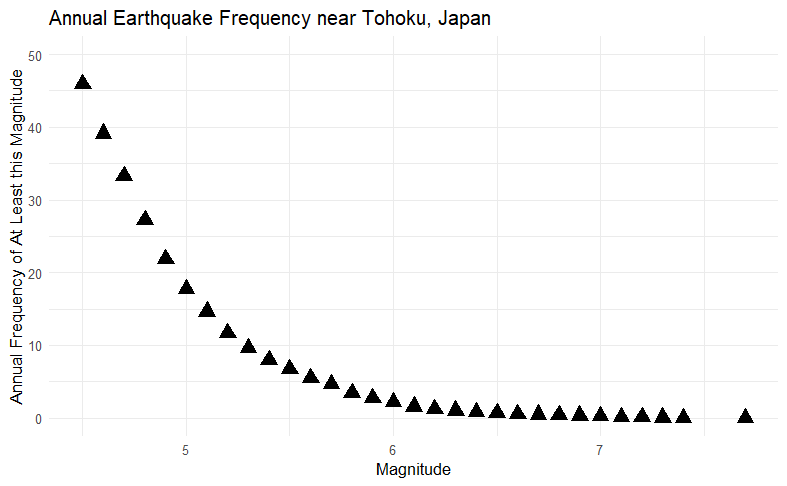
\includegraphics[width=0.5\linewidth]{Figures/tohoku_standardscale.png}
    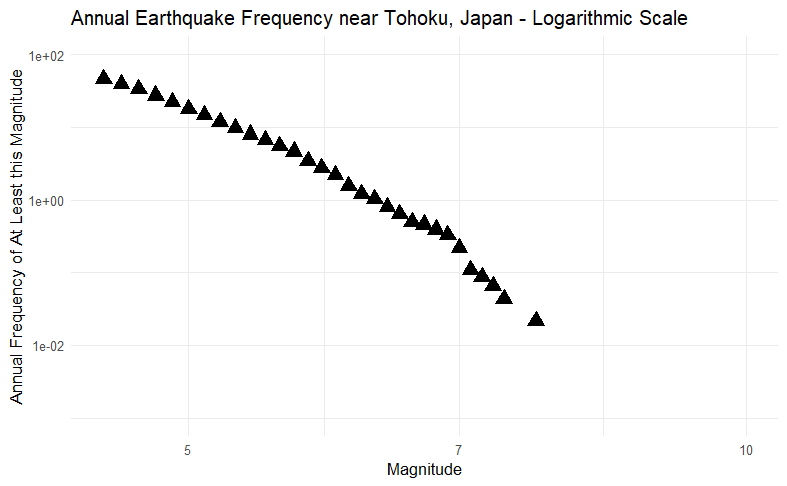
\includegraphics[width=0.5\linewidth]{Figures/tohoku_logscale.png}
   % \vspace{-10pt}
    \caption{\footnotesize{Annual Tohoku earthquake frequencies of magnitude 4.5 and above near displayed on the standard scale (left) and the logarithmic scale(right).}}
    \label{tohoku_unfit}
\end{figure}


\begin{comment}
\hypertarget{linear-models-of-the-data}{%
\subsection{Linear models of the data}\label{linear-models-of-the-data}}
\end{comment}

It is apparent based on this visualization that the logarithmic scale is more suited for a linear model.  After transformation the data, a the model is fit using
\texttt{R}.

\begin{figure}[H]
    \center
    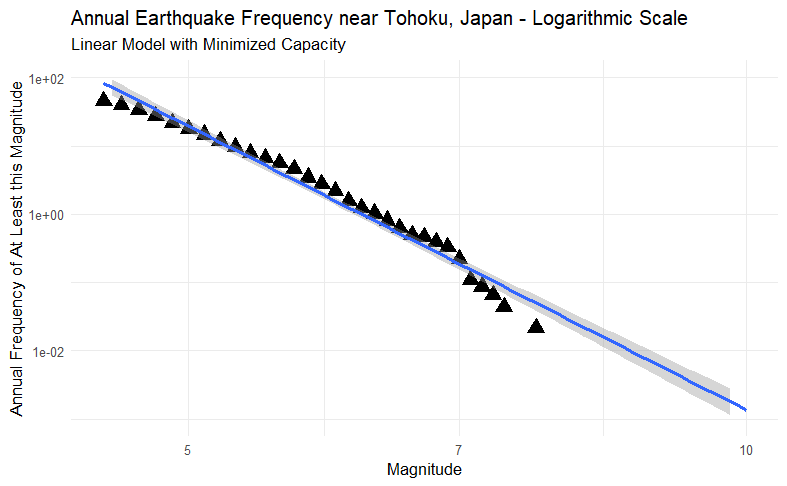
\includegraphics[width=0.65\linewidth]{Figures/tohoku_logscale_fit.png}
   % \vspace{-10pt}
    \caption{\footnotesize{The regression model of earthquake frequencies with minimal capacity.}}
    \label{tohoku_lm}
\end{figure}

\begin{Shaded}
\begin{Highlighting}[]
\CommentTok{\#transforming to the log scale}
\NormalTok{earthquakes\_log }\OtherTok{\textless{}{-}}\NormalTok{ earthquakes }\SpecialCharTok{\%\textgreater{}\%} \FunctionTok{mutate}\NormalTok{(}\AttributeTok{freqc =} \FunctionTok{log10}\NormalTok{(freqc)) }

\NormalTok{linear }\OtherTok{\textless{}{-}} \FunctionTok{lm}\NormalTok{(}\AttributeTok{data =}\NormalTok{ earthquakes\_log, }\AttributeTok{formula =}\NormalTok{ freqc }\SpecialCharTok{\textasciitilde{}}\NormalTok{ mag)}

\FunctionTok{summary}\NormalTok{(linear)}
\end{Highlighting}
\end{Shaded}

\begin{verbatim}
## 
## Call:
## lm(formula = freqc ~ mag, data = earthquakes_log)
## 
## Residuals:
##      Min       1Q   Median       3Q      Max 
## -0.19955 -0.06120  0.02396  0.06852  0.16566 
## 
## Coefficients:
##             Estimate Std. Error t value Pr(>|t|)    
## (Intercept)  6.38365    0.11513   55.45   <2e-16 ***
## mag         -1.01971    0.01895  -53.80   <2e-16 ***
## ---
## Signif. codes:  0 '***' 0.001 '**' 0.01 '*' 0.05 '.' 0.1 ' ' 1
## 
## Residual standard error: 0.0956 on 29 degrees of freedom
## Multiple R-squared:  0.9901, Adjusted R-squared:  0.9897 
## F-statistic:  2894 on 1 and 29 DF,  p-value: < 2.2e-16
\end{verbatim}


For completeness, this model shows that on average, for every 1.0 increase in magnitude, the lapsed time between earthquakes of \emph{at least} that magnitude is expected to increase by \(1/10^{-1.01971}\) = 10.4643 years.

For a magnitude 9.1 earthquake, the expected frequency would be one
every \(1/10^{(6.38365 - 1.01971 \cdot 9.1)}\) = 786.47 years.  This might be enough for Fukushima engineering officials to decide to design a nuclear reactor more resistant to higher magnitude earthquakes.  However, the graph contains a slight curvature that perhaps contains a better fit.  Below are two such options that display the capacity raised to second and third order polynomial.

\begin{figure}[H]
 %   \center
    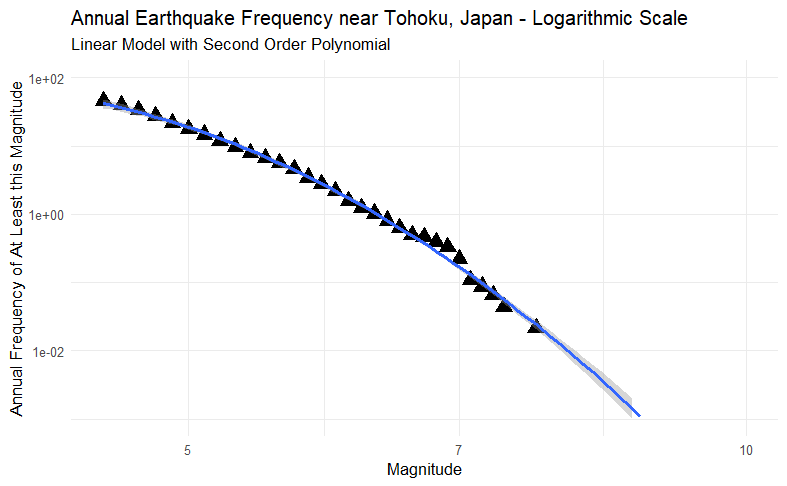
\includegraphics[width=0.5\linewidth]{Figures/tohoku_logscale_fit2.png}
    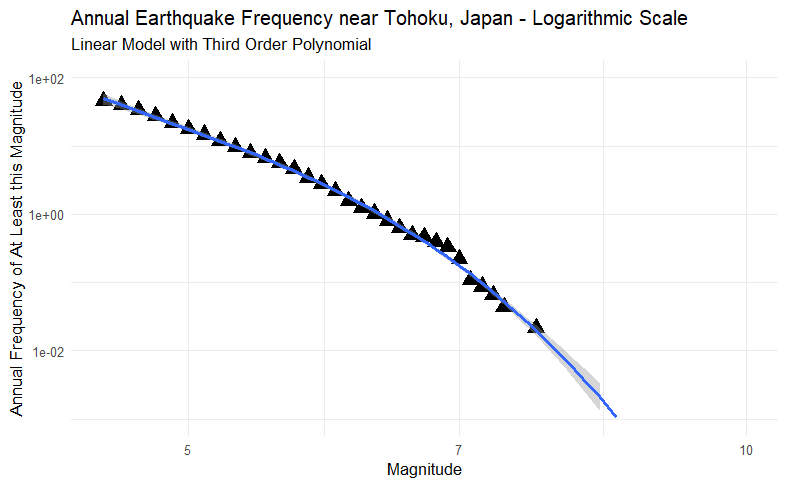
\includegraphics[width=0.5\linewidth]{Figures/tohoku_logscale_fit3.png}
   % \vspace{-10pt}
    \caption{\footnotesize{The regression model fit to the data with the second order polynomial (left) and the third order polynomial (right).}}
    \label{tohoku_lm23}
\end{figure}

By accounting for the curvature of the data, the predicted frequency of a data point outside of this interval changes dramatically.  A regression model inclusive of the second order polynomial predicts a magnitude 9.1 earthquake to occur every 5693.64 years; that with a third order polynomial to predict one every 24,721.19 years.

The following code outputs a data frame of polynomial levels and the relative expected interval of time between earthquakes of magnitude 9.1 or above in the Tohoku area.

\begin{Shaded}
\begin{Highlighting}[]
\NormalTok{capacity }\OtherTok{\textless{}{-}} \DecValTok{1}\SpecialCharTok{:}\DecValTok{8}
\NormalTok{prediction }\OtherTok{\textless{}{-}} \ConstantTok{NULL}

\ControlFlowTok{for}\NormalTok{(i }\ControlFlowTok{in}\NormalTok{ capacity)\{}
\NormalTok{  linear }\OtherTok{\textless{}{-}} \FunctionTok{lm}\NormalTok{(}\AttributeTok{data =}\NormalTok{ earthquakes\_log, }\AttributeTok{formula =}\NormalTok{ freqc }\SpecialCharTok{\textasciitilde{}} \FunctionTok{poly}\NormalTok{(mag,i))}
\NormalTok{  p }\OtherTok{\textless{}{-}} \FunctionTok{predict}\NormalTok{(linear, }\AttributeTok{newdata =} \FunctionTok{data.frame}\NormalTok{(}\AttributeTok{mag =} \FloatTok{9.1}\NormalTok{))}
\NormalTok{  prediction[i] }\OtherTok{\textless{}{-}} \DecValTok{1}\SpecialCharTok{/}\DecValTok{10}\SpecialCharTok{\^{}}\NormalTok{p}
\NormalTok{\}}
\FunctionTok{data.frame}\NormalTok{(capacity,prediction)}
\end{Highlighting}
\end{Shaded}

\begin{verbatim}
##   capacity    prediction
## 1        1  7.864653e+02
## 2        2  5.693638e+03
## 3        3  2.472119e+04
## 4        4  4.878898e+04
## 5        5  4.513788e-01
## 6        6  1.522366e-33
## 7        7 8.608668e-153
## 8        8  6.102735e-40
\end{verbatim}

As discussed in earlier sections, increasing the level at which the model fits the data comes with a very some meaningful caveat: it becomes less likely to extrapolate meaningful results.  By the fourth polynomial order, a magnitude 9.1 earthquake is expected only every 49,000 years.  By the fifth order, the predictions become useless and blatantly nonsensical.